\documentclass[11pt, a4paper]{scrartcl}

\usepackage[english]{babel}
\usepackage[paper=a4paper,bottom=3cm,top=3cm,left=2cm,right=2cm]{geometry}
\usepackage[T1]{fontenc}
\usepackage[utf8]{luainputenc}

\usepackage{graphicx}
\usepackage{wrapfig}

\usepackage{epstopdf}
\usepackage{amsmath}
\usepackage{amsfonts}

%\usepackage{biblatex}
%\usepackage{csquotes}

\title{An Introduction To Coaxial Rotors In Helicopter Design}
\author{Bjarne Oldenburg}
\date{\today}

\begin{document}

\maketitle

\section{Introduction}
A helicopter, named so by Ponton d' Amécourt, who derived the name from the greek elikoeioas, meaning winding (the word helix is derived from the very same origin), 
and pteron, which means wing, is - as implied by the etymological origin - defined as an aircraft using rotating airfoils as means of generating lift, thrust and any control inputs, and that is capable of controlled hover without forward movement.
The historical development of helicopters settled, after a large variety of designs in the early 1900s, on most helicopters using a larger main rotor, 
which generates vertical thrust and control inputs, combined with a smaller rear rotor to counteract the torque exerted on the helicopter.

\section{Mathematics}
Here is a test for github and also equations:
\begin{equation}
    E = mc^2
\end{equation}

\begin{equation}
    \frac{1}{2}mv^2 = mgh
\end{equation} 

We can also create matrices, such as:
\[
    A = \begin{pmatrix}
    1 & 2 & 3 \\
    4 & 5 & 6 \\
    7 & 8 & 9
    \end{pmatrix}
\]

\section{Figures}
Below is an example of an image. Make sure to have an image in the same directory as this .tex file and replace `example-image.png` with the name of your image file.

\begin{figure}[!ht]
    \centering
    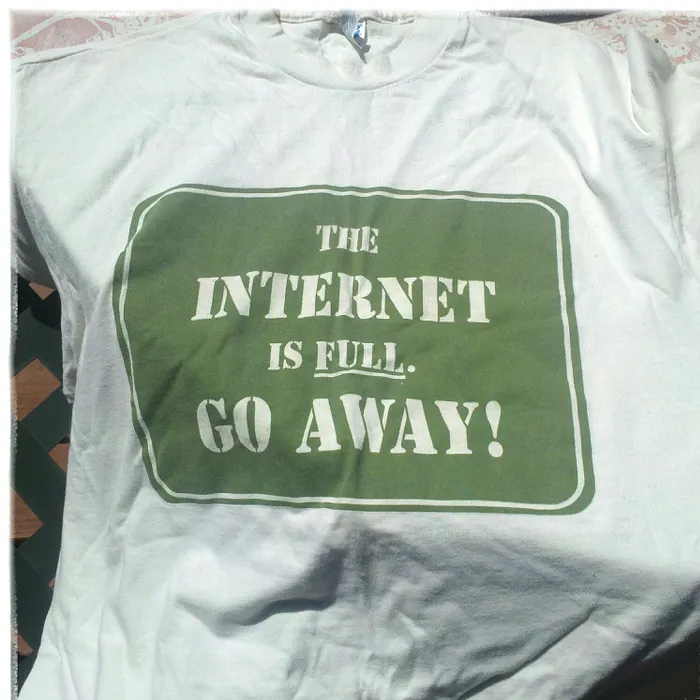
\includegraphics[width=0.5\textwidth]{test.png}
    \caption{This is a test image.}
    \label{fig:testimage}
\end{figure}

\section{References and Links}

\section{Conclusion}
If everything works fine, your LaTeX setup is working perfectly!

\end{document}